\documentclass[17pt]{beamer}
%\documentclass[handout]{beamer} %Makes Handouts
\usetheme{Singapore} %Gray with fade at top
\useoutertheme[subsection=false]{miniframes} %Supppress subsection in header
\useinnertheme{rectangles} %Itemize/Enumerate boxes
\usecolortheme{seagull} %Color theme
\usecolortheme{rose} %Inner color theme

\definecolor{light-gray}{gray}{0.75}
\definecolor{dark-gray}{gray}{0.55}
\setbeamercolor{item}{fg=light-gray}
\setbeamercolor{enumerate item}{fg=dark-gray}

\setbeamertemplate{navigation symbols}{}
\setbeamertemplate{mini frames}{}
%\setbeamercovered{dynamics}
\setbeamerfont*{title}{size=\Large,series=\bfseries}
\setbeamerfont{footnote}{size=\tiny}

%\setbeameroption{notes on second screen} %Dual-Screen Notes
%\setbeameroption{show only notes} %Notes Output

\setbeamertemplate{frametitle}{\vspace{.5em}\bfseries\insertframetitle}
\newcommand{\heading}[1]{\noindent \textbf{#1}\\ \vspace{1em}}
\newcommand{\questions}{\frame{{\large Questions?}}}

\usepackage{bbding,color,multirow,times,ccaption,tabularx,graphicx,verbatim,booktabs}
\usepackage{colortbl} %Table overlays
\usepackage[english]{babel}
\usepackage[latin1]{inputenc}
\usepackage[T1]{fontenc}
\usepackage{lmodern}
\usepackage{alltt}

\usepackage{tikz}
\usetikzlibrary{shapes,arrows,decorations.pathreplacing,calc}


\author[]{Thomas J. Leeper}
\institute{
  Government Department\\London School of Economics and Political Science
}

\usepackage{multirow}

\setbeamertemplate{headline}
 {%
  \begin{beamercolorbox}{section in head/foot}
  \insertsectionnavigationhorizontal{\textwidth}{}{}
  \end{beamercolorbox}%
}

\title{Session IV\\Practical Issues}

\date[]{}

\begin{document}

\frame{\titlepage}

\frame{\tableofcontents}

\section[More Designs]{Beyond One-Shot Designs}
\frame{\tableofcontents[currentsubsection,subsubsectionstyle=hide]}

\frame{

\frametitle{{\normalsize Beyond One-shot Designs}}


\begin{itemize}\itemsep0.5em
\item Surveys can be used as a measurement instrument for a field treatment or a manipulation applied in a different survey panel wave
	\begin{enumerate}
	\item Measure effect duration in two-wave panel
	\item Solicit pre-treatment outcome measures in a two-wave panel
	\item Measure effects of field treatment in post-test only design
	\item Randomly encourage field treatment in pre-test and measure effects in post-test
	\end{enumerate}
\item<2-> Problems? Compliance \& nonresponse
\end{itemize}

}

\frame{

\frametitle{{\normalsize I. Effect Duration}}

\begin{itemize}\itemsep0.5em
\item Use a two- (or more-) wave panel to measure duration of effects
	\begin{itemize}
	\item T1: Treatment and outcome measurement
	\item T2+: Outcome measurement
	\end{itemize}
\item Two main concerns
	\begin{itemize}
	\item Attrition
	\item Panel conditioning
	\end{itemize}
\end{itemize}

}

\frame{

\frametitle{{\normalsize II. Within-Subjects Designs}}

\small

\begin{itemize}
\item Estimate treatment effects as a difference-in-differences
\item Instead of using the post-treatment mean-difference in $Y$ to estimate the causal effect, use the difference in pre-post differences for the two groups:
	\begin{align*}
	(\hat{Y}_{0,t+1} - \hat{Y}_{0,t}) - (\hat{Y}_{j,t+1} - \hat{Y}_{j,t})
	\end{align*}
\item<2-> Advantageous because variance for paired samples decreases as correlation between $t_0$ and $t_1$ observations increases
\end{itemize}

}


\frame{
	\begin{center}
	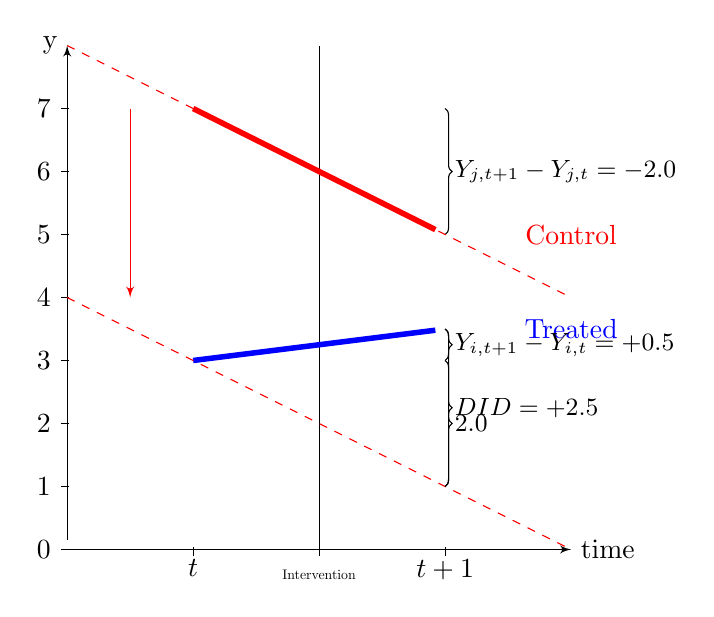
\begin{tikzpicture}[>=latex', scale=0.8]
        \draw[->] (0,0) node (origin) {}  -- (8,0) node[right] (xaxis) {time};
        \draw[->] (origin) -- (0,8) node[left] (yaxis) {y};
        % x ticks
        \foreach \x in {2,4,6}
        	\draw (\x,1pt) -- (\x,-3pt) node[anchor=north] {};
        \draw (2,0) node[below] (before) {$t$};
        \draw (6,0) node[below] (after) {$t+1$};
        \draw (4,-0.25) node[below, scale=0.5] (IV) {Intervention};
        % y ticks
        \foreach \y in {0,...,7}
             \draw (1pt,\y) -- (-3pt,\y) node[anchor=east] {$\y$};
        % intervention
        \draw (4,0) -- (4,8);

        % line
        \draw<2-> (6,3.5) node (tr) {};
        \draw<3-> (6,5) node (ctrl) {};
        \draw<2-3>[blue] (8,3.5) node (trlab) {Treated};
        \draw<3-3>[red] (8,5) node (ctrllab) {Control};        
        \draw<2->[blue, line width=2pt] (2,3) -- (tr);
        \draw<3->[red, line width=2pt] (2,7) -- (ctrl);
        
        % diffs
        \draw<4-6>[right,decorate,decoration={brace,mirror}] 
        	(6,3) -- (6,3.5) node[right, pos=0.5] (idiff) {\small $Y_{i,t+1} - Y_{i,t} = +0.5$};
        \draw<4-6>[right,decorate,decoration={brace}] 
            (6,7) -- (6,5) node[right, pos=0.5] (jdiff) {\small $Y_{j,t+1} - Y_{j,t} = -2.0$};
        
        % trends
        \draw<5-6>[red,->] (1,7) -- (1,4);
        \draw<5->[red, dashed] (0,8) -- (8,4);
        \draw<5->[red, dashed] (0,4) -- (8,0);
        \draw<6>[right,decorate,decoration={brace}] 
            (6,3) -- (6,1) node[right, pos=0.5] (idiff2) {\small $2.0$};
        \draw<7>[right,decorate,decoration={brace}] 
            (6,3.5) -- (6,1) node[right, pos=0.5] (idiff2) {\small $DID = +2.5$};
                        
        
    \end{tikzpicture}
    \end{center}
}


\frame{

	\frametitle{{\normalsize Threats to Validity}}
	
	\small
	
	As soon as time comes into play, we have to worry about threats to validity.\footnote{Shadish, Cook, and Campbell (2002)}
	
	\begin{enumerate}
	\item<2-> History (simultaneous cause)
	\item<3-> Maturation (time trends)
	\item<4-> Testing (observation changes respondents)
	\item<5-> Instrumentation (changing operationalization)
	\item<6-> Instability (measurement error)
	\item<7-> Attrition
	\end{enumerate}
}






\frame{

\frametitle{{\normalsize III. Randomized Field Treatment}}

\small

\begin{itemize}\itemsep-0.2em
\item Examples:
	\begin{enumerate}
	\item<2-> Citizens randomly sent a letter by post encouraging them to reduce water usage
	\item<3-> Different local media markets randomly assigned to receive different advertising
	\end{enumerate}
\item<4-> Survey is used to measure outcomes, when treatment assignment is already known
\item<5-> Issues
	\begin{itemize}
	\item<6-> Nonresponse
	\item<6-> Noncompliance
	\end{itemize}
\end{itemize}

}

\frame{
\frametitle{Noncompliance}

\small

\begin{itemize}
\item Compliance is when individuals receive and accept the treatment to which they are assigned
\item Noncompliance:\\{\small ``when subjects who were assigned to receive the treatment go untreated or when subjects assigned to the control group are treated'' \footnote{Gerber \& Green. 2012. \textit{Field Experiments}, p.132.}}
\item This causes problems for our analysis because factors other than randomization explain why individuals receive their treatment
\item Lots of methods for dealing with this, but the consequence is generally reduced power
\end{itemize}
}

\frame{
\frametitle{Asymmetric Noncompliance}

\small

\begin{itemize}\itemsep0.25em
\item Noncompliance \textit{asymmetric} if only in one group
\item We can ignore non-compliance and analyze the ``intention to treat'' effect, which will underestimate our effects because some people were not treated as assigned\\
	$ITT = \overline{Y}_1 - \overline{Y}_0$
\item We can use ``instrumental variables'' to estimate the ``local average treatment effect'' (LATE) for those that complied with treatment:\\
	$LATE = \frac{ITT}{Percent Compliant}$
\item We can ignore randomization and analyze data ``as-treated'', but this makes our study no longer an experiment
\end{itemize}
}

\frame{
	\frametitle{{\large Local Average Treatment Effect}}
	\small
	\begin{itemize}\itemsep0.2em
	\item IV estimate is \textit{local} to the variation in $X$ that is due to variation in $D$
	\item LATE is effect for those who \textit{comply}
	\item Four subpopulations:
		\begin{itemize}\footnotesize
		\item Compliers: $X = 1$ only if $D = 1$
		\item Always-takers: $X = 1$ regardless of $D$
		\item Never-takers: $X = 0$ regardless of $D$
		\item Defiers: $X = 1$ only if $D = 0$
		\end{itemize}
	\item Exclusion restriction! Monotonicity!
	\end{itemize}
}

\frame{
\frametitle{Two-Sided Noncompliance}
\begin{itemize}\itemsep1em
\item Two-sided noncompliance is more complex analytically
\item Stronger assumptions are required to analyze it and we won't discus them here
\item Best to try to develop a better design to avoid this rather than try to deal with the complexities of analyzing a broken design
\end{itemize}
}





\frame{

\frametitle{{\normalsize IV. Treatment Encouragement}}

\small

\begin{itemize}\itemsep-0.2em
\item Design:
	\begin{itemize}
	\item T1: Encourage treatment
	\item T2: Measure effects
	\end{itemize}
\item Examples:
	\begin{enumerate}
	\item Albertson and Lawrence\footnote{Albertson \& Lawrence. 2009. ``After the Credits Roll.'' \textit{American Politics Research} 37(2): 275--300. \href{http://doi.org/10.1177/1532673X08328600}{10.1177/1532673X08328600}.}
	\end{enumerate}
\item<2-> Issues
	\begin{itemize}
	\item<3-> Nonresponse
	\item<3-> Noncompliance
	\end{itemize}
\end{itemize}

}


\frame{

\frametitle{{\normalsize Treatment Noncompliance}}

\begin{itemize}\itemsep0.5em
\item<2-> Several strategies
	\begin{itemize}
	\item ``As treated'' analysis
	\item ``Intention to treat'' analysis
	\item Estimate a LATE
	\end{itemize}
\end{itemize}

}

\questions


\frame{}

\section[Quiz]{Handling ``Broken'' Experiments}
\frame{\tableofcontents[currentsection]}

\frame{

\Large

\begin{center}
Quiz time!
\end{center}

}


\frame{
\frametitle{Compliance}

\large

\begin{enumerate}\itemsep0.5em
\item<1-> What is compliance?
\item<2-> How can we analyze experimental data when there is noncompliance?
\end{enumerate}
}

\frame{
\frametitle{Balance testing}

\normalsize

\begin{enumerate}\itemsep0.5em
\item<1-> What does randomization ensure about the composition of treatment groups?
\item<2-> What can we do if we find a covariate imbalance between groups?
\item<3-> How can we avoid this problem entirely?
\end{enumerate}
}


\frame{
\frametitle{Nonresponse and Attrition}

\large

\begin{enumerate}\itemsep0.5em
\item<1-> Do we care about outcome nonresponse in experiments?
\item<2-> How can we analyze experimental data when there is outcome nonresponse or post-treatment attrition?
\end{enumerate}
}


\frame{
\frametitle{Manipulation checks}

\large

\begin{enumerate}\itemsep0.5em
\item<1-> What is a manipulation check? What can we do with it?
\item<2-> What do we do if some respondents ``fail'' a manipulation check?
\end{enumerate}
}



\frame{
\frametitle{Null effects}

\large

\begin{enumerate}\itemsep0.5em
\item<1-> What should we do if we find our estimated $\widehat{SATE} = 0$?
\item<2-> What does it mean for an experiment to be \textit{underpowered}?
\item<3-> What can we do to reduce the probability of obtaining an (unwanted) ``null effect''?
\end{enumerate}
}


\frame{
\frametitle{Effect heterogeneity}

\large

\begin{enumerate}\itemsep0.5em
\item<1-> What should we do if, post-hoc, we find evidence of effect heterogeneity?
\item<2-> What can we do pre-implementation to address possible heterogeneity?
\end{enumerate}
}


\frame{
\frametitle{Representativeness}

\large

\begin{enumerate}\itemsep0.5em
\item<1-> Under what conditions is a design-based, probability sample necessary for experimental inference?
\item<2-> What kind of causal inferences can we draw from an experiment on a descriptively unrepresentative sample?
\end{enumerate}
}

\frame{
\frametitle{Peer Review}

\large

\begin{enumerate}\itemsep0.5em
\item<1-> What should we do if a peer reviewer asks us to ``control'' for covariates in the analysis?
\item<2-> What should we do if a peer reviewer asks us to include or exclude particular respondents from the analysis?
\end{enumerate}
}


\questions



\section{Research Ethics}
\frame{\tableofcontents[currentsection]}

\frame{
\frametitle{History: Key Moments}

\small

\begin{enumerate}
\item Tuskegee (1932-1972) and Guatemala (1946-1948) Studies
\item Nuremberg Code (1947)
\item Helsinki Declaration (1964)
\item U.S. 45 CFR 46 (1974) and ``Common Rule'' (1991)
\item The Belmont Report (1979)
\item EU Data Protection Directive (1995; 2012)
	\begin{itemize}
	\item UK Data Protection Act (1998)
	\end{itemize}
\end{enumerate}
}


\frame{
	\frametitle{Helsinki Declaration}
	
	\small
	\begin{itemize}
	\item Adopted by the World Medical Association in 1964\footnote{\url{http://www.bmj.com/content/2/5402/177}}
	\item Narrowly focused on medical research
	\item Expanded the Nuremberg Code
		\begin{itemize}
		\item Relaxed consent requirements
		\item Risks should not exceed benefits
		\item Institutionalization of ethics oversight
		\end{itemize}
	\item<2-> Do these rules apply to non-medical research?
	\end{itemize}

}

\frame{
	\frametitle{The Belmont Report}
	
	\small
	\begin{itemize}
	\item Commissioned by the U.S. Government in 1979\footnote{\url{http://www.hhs.gov/ohrp/humansubjects/guidance/belmont.html}}
	\item Three overarching principles:
		\begin{enumerate}
		\item Respect for persons
		\item Beneficence
		\item Justice
		\end{enumerate}
	\item Three policy implications:
		\begin{itemize}
		\item Informed consent
		\item Assessment of risks/benefits
		\item Care for vulnerable populations
		\end{itemize}
	\end{itemize}

}

\frame{
\frametitle{Benefits and Harm}
	\begin{itemize}\itemsep1em
	\item What is a ``benefit''?
	\item What is a ``harm''?
	\item How do we balance the two?
	\end{itemize}
}


\frame{

\frametitle{Ethical Considerations}

\begin{itemize}
\item Most ethical issues are not unique to \textit{experimental} social science
\item Some especially important issues:
	\begin{enumerate}
	\item Randomization
	\item Informed consent
	\item Privacy
	\item Deception
	\item Publication bias
	\end{enumerate}
\end{itemize}

}

\frame{

\frametitle{I. Randomization}

\begin{itemize}
\item Is it ethical to randomize?
\end{itemize}

}



\frame{
	\frametitle{II. Informed Consent}
	\begin{itemize}
	\item Persons must consent to being a research subject
	\item<2-> What this means in practice is complicated
		\begin{itemize}
		\item What is consent?
		\item What is ``informed'' consent?
		\item What exactly do they have to consent to?
		\end{itemize}
	\item<3-> Cross-national variations
		\begin{itemize}
		\item Consent forms required in U.S.
		\item Not required in UK
		\end{itemize}
	\end{itemize}

}


\frame{
	\frametitle{III. Privacy}
	\begin{itemize}\itemsep0.5em
	\item Under EU Data Protection Directive (1995), data can be processed when:
		\begin{itemize}
		\item Consent is given
		\item Data are used for a ``legitimate'' purpose
		\item Anonymous or confidential
		\end{itemize}
	\item Data cannot leave the EU except under conditions
	\end{itemize}

}

\frame{
	\frametitle{III. Privacy}
	\begin{itemize}\itemsep1em
	\item Experimental might be additionally sensitive
	\item<2-> Answers reflect ``manipulated'' attitudes, behaviors, perceptions, etc. that respondents may not have given in another setting
	\end{itemize}

}



\frame{

\frametitle{IV. Deception}

\begin{itemize}
\item Major distinction between psychology tradition and economics tradition\footnote{Dickson, E. 2011. ``Economics versus Psychology Experiments.'' \textit{Cambridge Handbook of Experimental Political Science}.}
	\begin{itemize}
	\item Purpose of the study
	\item Purpose of specific items or tasks
	\item Order or length of questionnaire
	\end{itemize}
\item<2-> Psychologists focus on \textit{debriefing}
\item<3-> Within economics, norms about \textit{acts of omission} versus \textit{acts of commission}
	\begin{itemize}
	\item<4-> Omission: In a multi-round trust game, an additional round is added
	\item<5-> Commission: Telling respondents it is a dictator game, but it is actually a trust game
	\end{itemize}
\end{itemize}


}


\frame{

\frametitle{V. Publication Bias}

\begin{itemize}\itemsep0.5em
\item Publication bias not typically discussed as an ethical question
\item<2-> If studies are meant to policy or practical implications, then we care about PATE or a set of CATEs, including whether their effects are positive, negative, or zero.
\item<3-> Publication bias (toward ``significant'' results) invites wasting resources on treatments that actually don't work
\end{itemize}

}



\frame{
	\frametitle{{\normalsize Lots of Other Ethical Questions}}
	\begin{enumerate}
	\item<2-> Funding
	\item<3-> Independence and Politicization
	\item<4-> Vulnerable populations (e.g. children, sick)
	\item<5-> Incentives
	\item<6-> Cross-national research
	\item<7-> End uses/users of research
	\item<8-> Others\dots
	\end{enumerate}
}

\questions

\section{Conclusion}
\frame{\tableofcontents[currentsection]}

\frame{

\frametitle{Learning Outcomes}

\small

By the end of the week, you should be able to\dots

\begin{enumerate}
\item<2-> Explain how to analyze experiments quantitatively.
\item<3-> Explain how to design experiments that speak to relevant research questions and theories.
\item<4-> Evaluate the uses and limitations of several common survey experimental paradigms.
\item<5-> Identify practical issues that arise in the implementation of experiments and evaluate how to anticipate and respond to them.
\end{enumerate}

}


\frame{
	\frametitle{Wrap-up}
	\begin{itemize}
	\item Thanks to all of you!
	\item Stay in touch (\href{mailto:t.leeper@lse.ac.uk}{t.leeper@lse.ac.uk})
	\item Good luck with your research!
	\end{itemize}
}


\appendix


\end{document}
